\documentclass[../ZF_Wing.tex]{subfiles}

\begin{document}



\title\textbf{Einordnung:\\}
\begin{figure}[H]
\centering
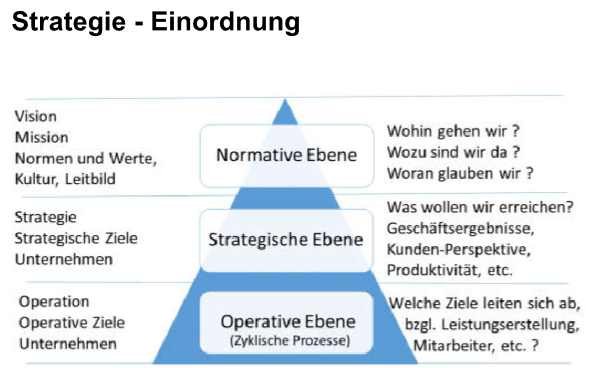
\includegraphics[width=0.3\textwidth]{Resources/Image/StrategieEinordnung.png}
\caption{\label{fig:StrategieEinordnung}StrategieEinordnung.}
\end{figure}

\title\textbf{Für Management-Entscheide:\\}
\begin{figure}[H]
\centering
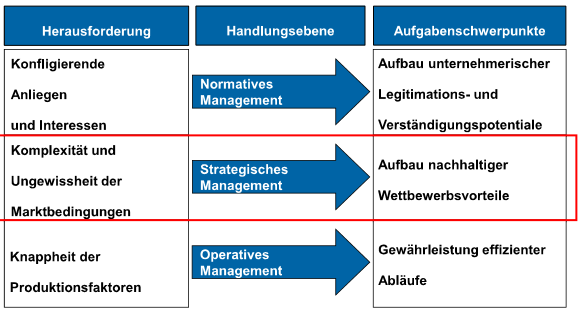
\includegraphics[width=0.3\textwidth]{Resources/Image/ManagementEntscheide.png}
\caption{\label{fig:ManagementEntscheide}ManagementEntscheide.}
\end{figure}


\subsection{Strategiefindungsprozess}
\paragraph{In vier Schritten:}
\begin{enumerate}
\item Strategische Analyse
\item Strategische Planung
\item Strategische Umsetzung
\item Strategische Messung
\end{enumerate}
\pagebreak
\subsection{Die strategische Analyse}
\subparagraph{Drei Modellen:}
\begin{itemize}
\item SWOT-Analyse
\item PESTEL-Analyse
\item 5-Forces Modell von Porter
\end{itemize}

\subparagraph{Faktoren, die Analyse beeinflussen\\}
\begin{figure}[H]
\centering
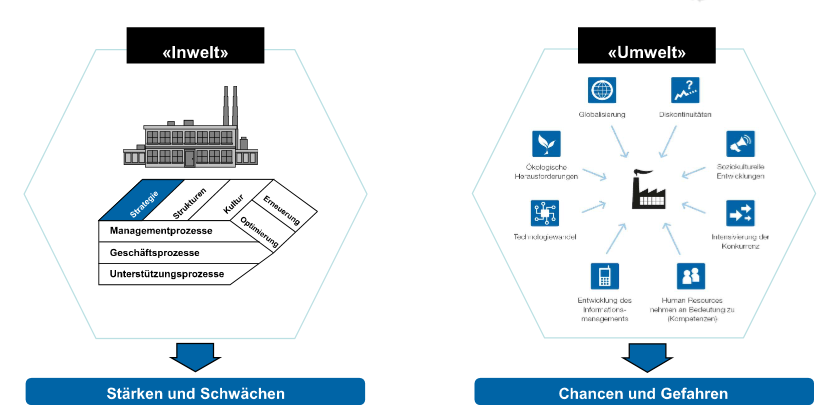
\includegraphics[width=0.3\textwidth]{Resources/Image/FaktorenEinfluss.png}
\caption{\label{fig:FaktorenEinfluss}FaktorenEinfluss.}
\end{figure}

\subsubsection{SWOT-Analyse:}
\begin{figure}[H]
\centering
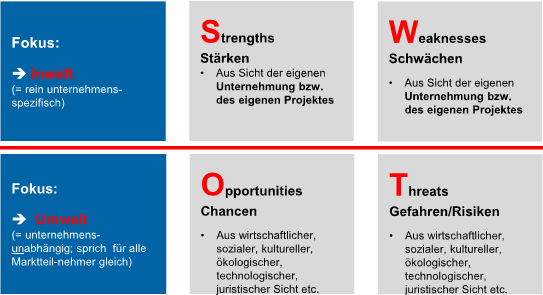
\includegraphics[width=0.3\textwidth]{Resources/Image/SwotAnalyse.png}
\caption{\label{fig:SwotAnalyse}SwotAnalyse.}
\end{figure}

\subparagraph{Kern-Kompetenzen:}

Kompetenz als Wettbewerbsvorteil
\begin{itemize}
\item Wertvoll
\item Selten
\item Nicht oder schwer imitierbar
\item Nicht substituierbar
\end{itemize}


\paragraph{Unternehmensanalyse Beispiel Easyjet \\ \\}

\begin{tabular}{|l|c|}
\hline
\rule[-1ex]{0pt}{2.5ex} 
\textbf{Strenghts} & \textbf{Weaknesses} \\ 
\hline 
\rule[-1ex]{0pt}{2.5ex}
Moderne Flugzeuge mit tiefen Betriebskosten & Keine Interkontinentalflüge \\ 
\hline 
\rule[-1ex]{0pt}{2.5ex}
Ersten Fluggesellschaften,Internetplattform zum Buchen & Gewisse (teure)Flughäfen  nicht Streckennetz \\ 
\hline
\rule[-1ex]{0pt}{2.5ex} 
Einheitliches Angebot (Bloss Ecenomy Class etc) &  \\ 
\hline
\rule[-1ex]{0pt}{2.5ex}
\end{tabular} \\ \\


\begin{tabular}{|l|l|}
\hline 
\rule[-1ex]{0pt}{2.5ex}
\textbf{Opportunities} & \textbf{Threats} \\ 
\hline 
\rule[-1ex]{0pt}{2.5ex} Wetter(Schlecht in CH zu Gut Ausland) & Covid-19 Reisebeschränkungen \\ 
\hline 
\rule[-1ex]{0pt}{2.5ex} Trend Wochenend Städtereisen & Verteuerung Treibstoffkosten \\ 
\hline 
\rule[-1ex]{0pt}{2.5ex} Grössere Flugzeuge & Höhere Flughafentaxen \\ 
\hline 
\rule[-1ex]{0pt}{2.5ex} Steigender Wohlstand & Verlängerung Nachtflugsperre europ.Flughafen \\ 
\hline 
\rule[-1ex]{0pt}{2.5ex}  & Neue Billig-Airlines \\ 
\hline 
\end{tabular} 
\\
\\

\title\textbf{Die vier abgeleiteten Grundstrategieansätze: \\}
\begin{figure}[H]
\centering
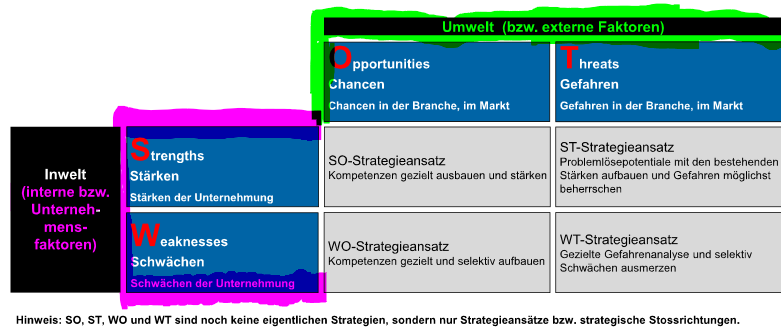
\includegraphics[width=0.3\textwidth]{Resources/Image/GrundstrategieAnsaetze.png}
\caption{\label{fig:GrundstrategieAnsaetze}GrundstrategieAnsaetze.}
\end{figure}


\subsubsection{PESTEL-Analyse}

Untersucht den Einfluss der sechs \textbf{externen} Umweltfaktoren \\
\begin{figure}[H]
\centering
\includegraphics[width=0.3\textwidth]{Resources/Image/Pestelanalyse.png}
\caption{\label{fig:Pestelanalyse}Pestelanalyse.}
\end{figure}




\subsubsection{5 Kräfte Modell von Porter}

Untersucht den Markt. \\

\begin{figure}[H]
\centering
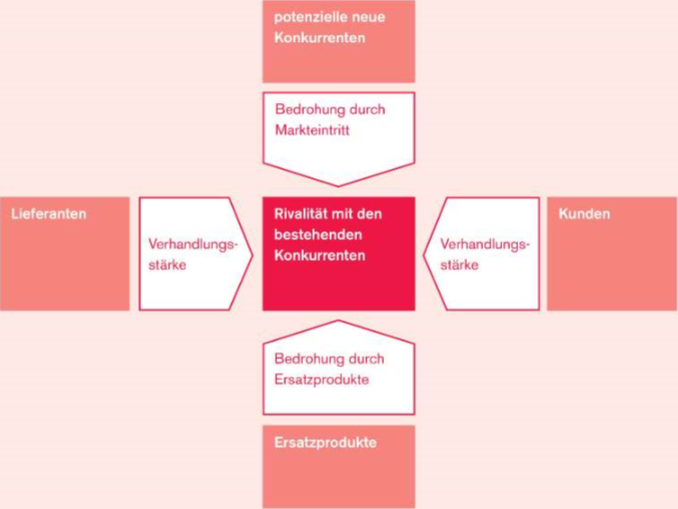
\includegraphics[width=0.3\textwidth]{Resources/Image/Porteranalyse.png}
\caption{\label{fig:Porteranalyse}Porteranalyse.}
\end{figure}


\begin{figure}[H]
\centering
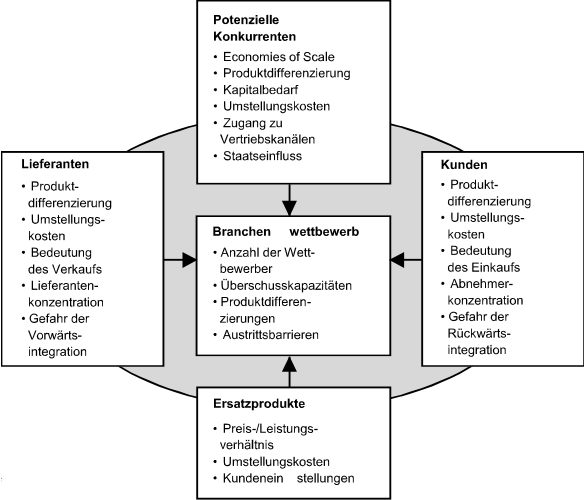
\includegraphics[width=0.3\textwidth]{Resources/Image/ZFPorter.png}
\caption{\label{fig:ZFPorter}ZFPorter.}
\end{figure}

\title\textbf{Branchenanalyse EasyJet\\}

\begin{figure}[H]
\centering
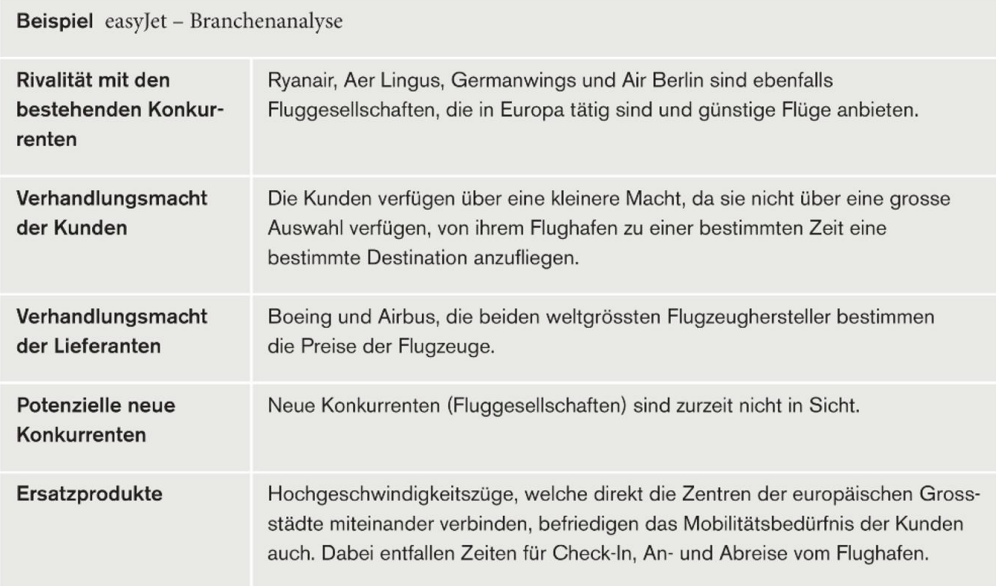
\includegraphics[width=0.3\textwidth]{Resources/Image/Branchenanalyse.png}
\caption{\label{fig:Branchenanalyse}Branchenanalyse.}
\end{figure}


\title\textbf{Entwicklung einer Strategie \\}
\begin{figure}[H]
\centering
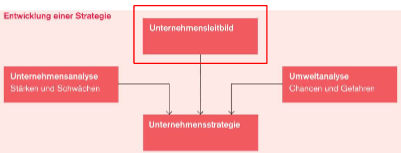
\includegraphics[width=0.3\textwidth]{Resources/Image/Strategieentwicklung.png}
\caption{\label{fig:Strategieentwicklung}Strategieentwicklung.}
\end{figure}


\title\textbf{Unternehmensleitbild \\}
\begin{figure}[H]
\centering
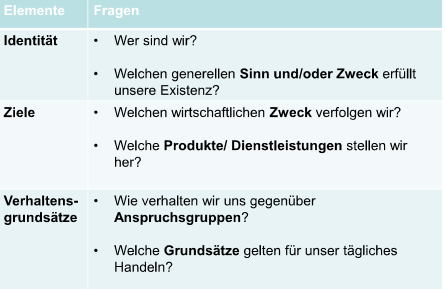
\includegraphics[width=0.3\textwidth]{Resources/Image/Unternehmensleitbild.png}
\caption{\label{fig:Unternehmensleitbild}Unternehmensleitbild.}
\end{figure}
\pagebreak
\title\textbf{Unternehmensstrategie\\}
\begin{figure}[H]
\centering
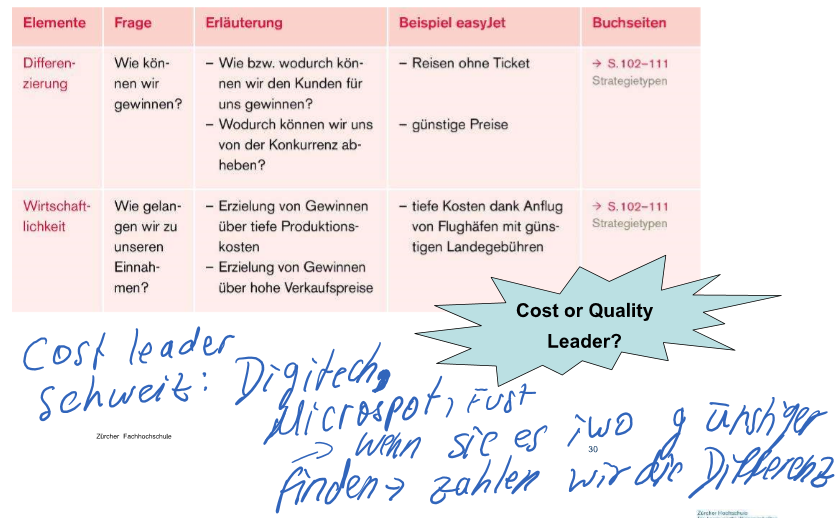
\includegraphics[width=0.3\textwidth]{Resources/Image/Unternehmensstrategie.png}
\caption{\label{fig:Unernehmungsstrategie}Unternehmensstrategie.}
\end{figure}



\subsection{Die Strategische Planung}

Hier geht es um die \textbf{Strategieformulierung und -auswahl \\}

\paragraph{zwei Modelle: \\}
\begin{enumerate}
\item 4-Branchenwettbewerbsstrategien nach Porter
\item 4-Produkt-Markt-Strategien nach Ansoff
\end{enumerate}


\begin{Large}
\title\textbf{4-Branchenwettbewerbsstrategien nach Porte \\}
\end{Large}

\begin{figure}[H]
\centering
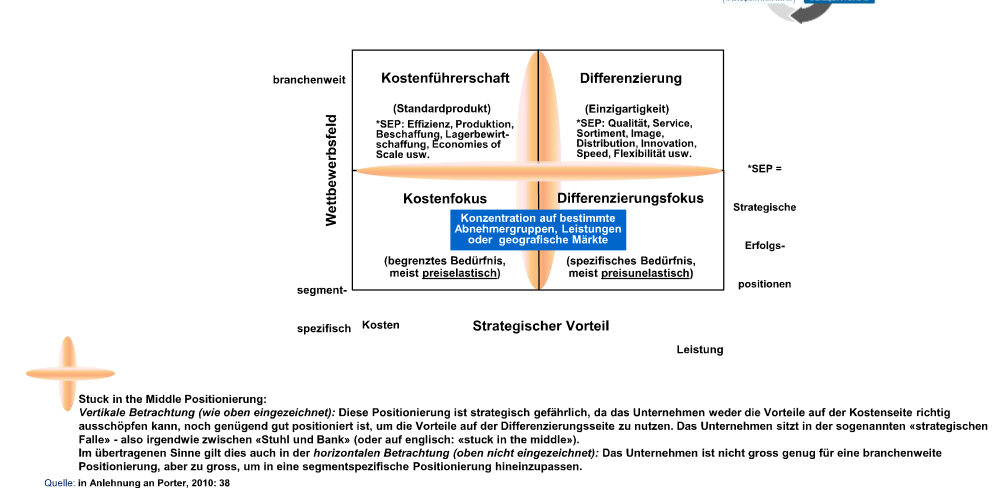
\includegraphics[width=0.3\textwidth]{Resources/Image/PorterWettbewerbstrategie.png}
\caption{\label{fig:PorterWettbewerbstrategie}PorterWettbewerbstrategie.}
\end{figure}



\begin{Large}
\title\textbf{4-Produkt-Markt-Strategien nach Ansoff \\}
\end{Large}

\begin{figure}[H]
\centering
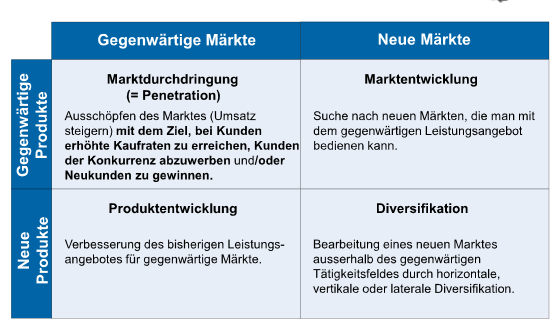
\includegraphics[width=0.3\textwidth]{Resources/Image/Ansoff.png}
\caption{\label{fig:Ansoff}Ansoff.}
\end{figure}
\pagebreak
\title\textbf{Die drei Stossrichtungen und ihre Erfolgsaussichten \\}

\begin{figure}[H]
\centering
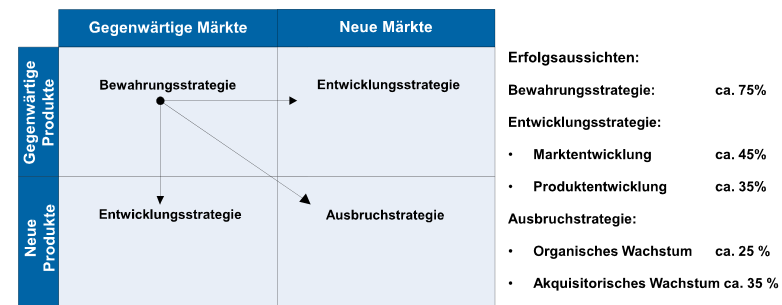
\includegraphics[width=0.3\textwidth]{Resources/Image/Stossrichtungen.png}
\caption{\label{fig:Stossrichtungen}Stossrichtungen.}
\end{figure}

\title\textbf{Marktdurchdringung\\}

\begin{figure}[H]
\centering
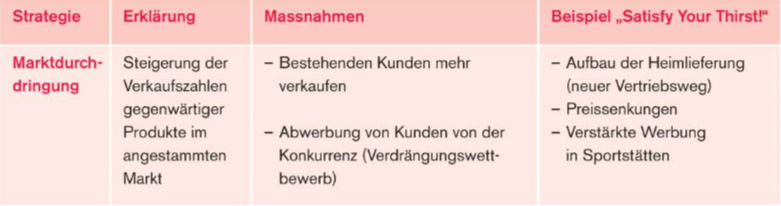
\includegraphics[width=0.3\textwidth]{Resources/Image/Marktdurchdringung.png}
\caption{\label{fig:Marktdurchdringung}Marktdurchdringung.}
\end{figure}


\title\textbf{Marktentwicklung\\}

\begin{figure}[H]
\centering
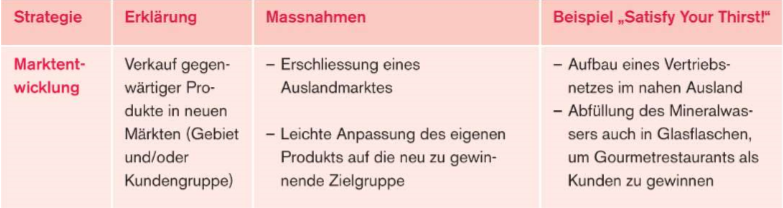
\includegraphics[width=0.3\textwidth]{Resources/Image/Marktentwicklung.png}
\caption{\label{fig:Marktentwicklung}Marktentwicklung.}
\end{figure}


\title\textbf{Produktentwicklung\\}

\begin{figure}[H]
\centering
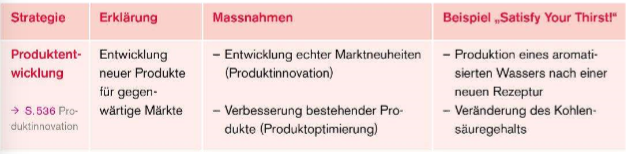
\includegraphics[width=0.3\textwidth]{Resources/Image/Produktentwicklung.png}
\caption{\label{fig:Produktentwicklung}Produktentwicklung.}
\end{figure}


\title\textbf{Diversifikation\\}
\begin{figure}[H]
\centering
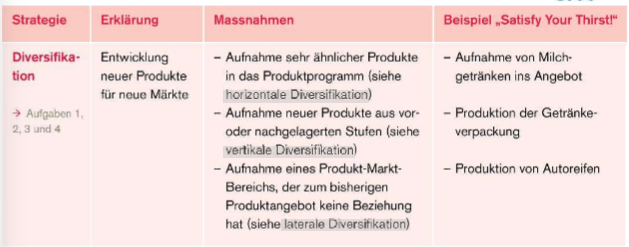
\includegraphics[width=0.3\textwidth]{Resources/Image/Diversifikation.png}
\caption{\label{fig:Diversifikation}Diversifikation.}
\end{figure}


















































\end{document}